\documentclass{article}
\usepackage{float,amsmath}
\usepackage{graphicx}
\usepackage{color}
\usepackage[a4paper,margin=2cm]{geometry}
\usepackage{hyperref}

%\setlength{\textwidth}{6.5in}

\begin{document}

\author{David DeBoer}
\title{HERA Dimensions} 
\maketitle

\section{Introduction}
This document provides details on dimensioning of the HERA element.  Section 1 details the hub and support spars.  Section 2 details the mesh.
Section 3 details the surface spars and bracing.  Section 4 details the feed height.  Actual dimensional values for Sections 1 - 3 are in the python scripts {\tt dims.py}, 
with values for South Africa, the UK and the US.  Section 4 includes the actual values specifically for South Africa.

\section{Hub and Support Spar}
\begin{figure}[H]
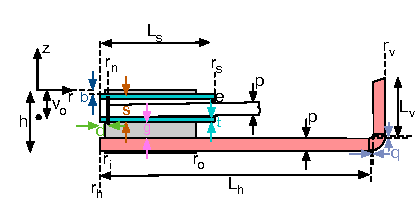
\includegraphics[width=0.8\textwidth]{hubdims.pdf}
\centering
\vspace{-.15in}
\caption{General dimensions of hub and support spar (colored light red).}
\label{fig:hubdims}
\end{figure}

\begin{tabular}{l l}
$h$          & height of hub \\
$v_o$      & distance of vertex from top of hub \\
$b$          & distance between top of hub and top of sleeve \\
$L_s$      & length of sleeve \\
$s$          & outer diameter of sleeve \\
$t$           & wall thickness of sleeve \\
$g$          & distance between bottom of sleeve and top of horizontal support spar \\
$d$          & distance between nail and the inner edge of the sleeve \\
$q$          & distance between 90$^o$ coupler spar and and orthogonal edge \\
$e$          & spacer-gap at outer edge of sleeve \\
$h_v$      & distance between top of horizontal support spar and lower edge of vertical support spar \\
$r_i$        & radial distance to inner edge of hub  \\
$r_o$       & radial distance to outer edge of hub  \\
$r_n$       & radial distance to nail  \\
$r_s$       & radial distance to end of sleeve  \\
$r_h$       & radial distance to inner edge of horizontal support \\
$L_h$      & length of horizontal support spar \\
$L_v$      & long length of vertical support spar \\
$F$          & focal length of parabola \\
$z$          & height z with 0 at top of hub \\
$r$           & radial distance with 0 at center of hub\\
$\theta(r)$& = $\tan^{-1}(r/2F)$
\end{tabular}
%\vspace{.in}

The hub is a concrete ``donut'' made up of two concentric rings with holes cut in to allow PVC spars to be positioned.  There are two sets of spar holes, each of which have twelve equi-spaced holes in the inner and outer rings.  There is another small hole $v_o$ from the top of the inner ring to accommodate a piece of rebar.  The bottom holes have diameter $p$ and the top holes have diameter $s$.  The bottom holes are centered $b+s+g+p/2$ from the top of the hub and the top holes are centered $b+s/2$ from the top.  The hub height is $h$.

\subsection{Sleeve and Vertex Offset}
To get the offset between the top of the hub and the vertex, we need to set the sleeve in one of two ways:

\vspace{.3in}
\noindent
{\bf 1:}  Given $s, t$, design the sleeve to the correct length $L_s$ (so $e=0$).
Matching the angle at the exit from the sleeve to the proper parabolic angle (see Sec. \ref{sec:derive}):
\begin{equation}
r_s = \frac{r_n + \sqrt{r_n^2 + 8(s - 2t - p)F}}{2}
\label{eq:sleeveExitAngle}
\end{equation}
Then $L_s = r_s - r_n + d$.

\vspace{0.2in}
\noindent
{\bf 2:}  Make a sleeve ($s, t, L_s$) then include a spacer $e$.  Then $r_s = L_s + r_n - d$ and 
\begin{equation}
e = (s - 2t - p) - \frac{r_s(r_s - r_n)}{2F}
\label{eq:spacer}
\end{equation}
\noindent
Then
\begin{equation}
v_o = b + t + e + \frac{r_s^2}{4F}
\end{equation}

\subsection{Parabolic Offsets from Top of Hub}
\noindent
Height from the top of the hub surface to the top of the spar ($z_t$) at radius $r$:
\begin{equation}
z_t(r) = \left(\frac{r^2}{4F}\right) - v_o
\end{equation}

\noindent
Height from the top of the hub surface to the bottom of the spar ($z_b$) at radius $r$:
\begin{equation}
z_b(r) = z_t - \left(\frac{p}{\cos\theta(r)}\right) = \left(\frac{r^2}{4F}\right) - \left(\frac{p}{\cos\theta(r)}\right) - v_o \approx \left[\frac{r^2}{4F(1+p/2F)}\right] - (v_o + p)
\end{equation}
 
\subsection{Vertical Support Spar}
\noindent
Length of the vertical support piece at the end of the support:
\begin{equation}
L_v = z_b(r_v) + b + s + g - q = \left(\frac{r_v^2}{4F}\right) - \left(\frac{p}{\cos\theta(r_v)}\right) - v_o + b + s + g - q
\end{equation}
where $r_v = r_h + L_h + q + p$.

\subsection{Some Derivations}
\label{sec:derive}
For Eq. \ref{eq:sleeveExitAngle}, note that the angle of spar in sleeve
\begin{equation}
\tan\theta_{exit} \approx \frac{s - 2t - p - e}{r_s-r_n}
\end{equation}
should match the angle at radius $r_s$ so 
\begin{equation}
\frac{s-2t-p-e}{r_s-r_n} = \frac{r_s}{2F}
\end{equation}
From which Equations \ref {eq:sleeveExitAngle} and \ref{eq:spacer} follow.

\section{Surface Mesh}
\vspace{-.5in}
\noindent
\begin{figure}[H]
\includegraphics[width=1.0\textwidth]{panels_all.pdf}
\centering
\vspace{-.15in}
\caption{Panel layout.  Bottom shows the (flat) arrangement as on antenna.}
\label{fig:panels}
\end{figure}
The surface are panels cut from galvanized and cross welded $\sim$6mm mesh coming from a standard width role of 1.22m, as shown in Figure \ref{fig:panels}.  There are 5 panel types, labelled A-E.  There are 12 A panels and 24 B-E panels.  One B panel is used as an access door.  The panels are overlapped as shown in the bottom of Figure \ref{fig:panels}, with an overlap width of $\rho_o = $100mm.
\begin{figure}[H]
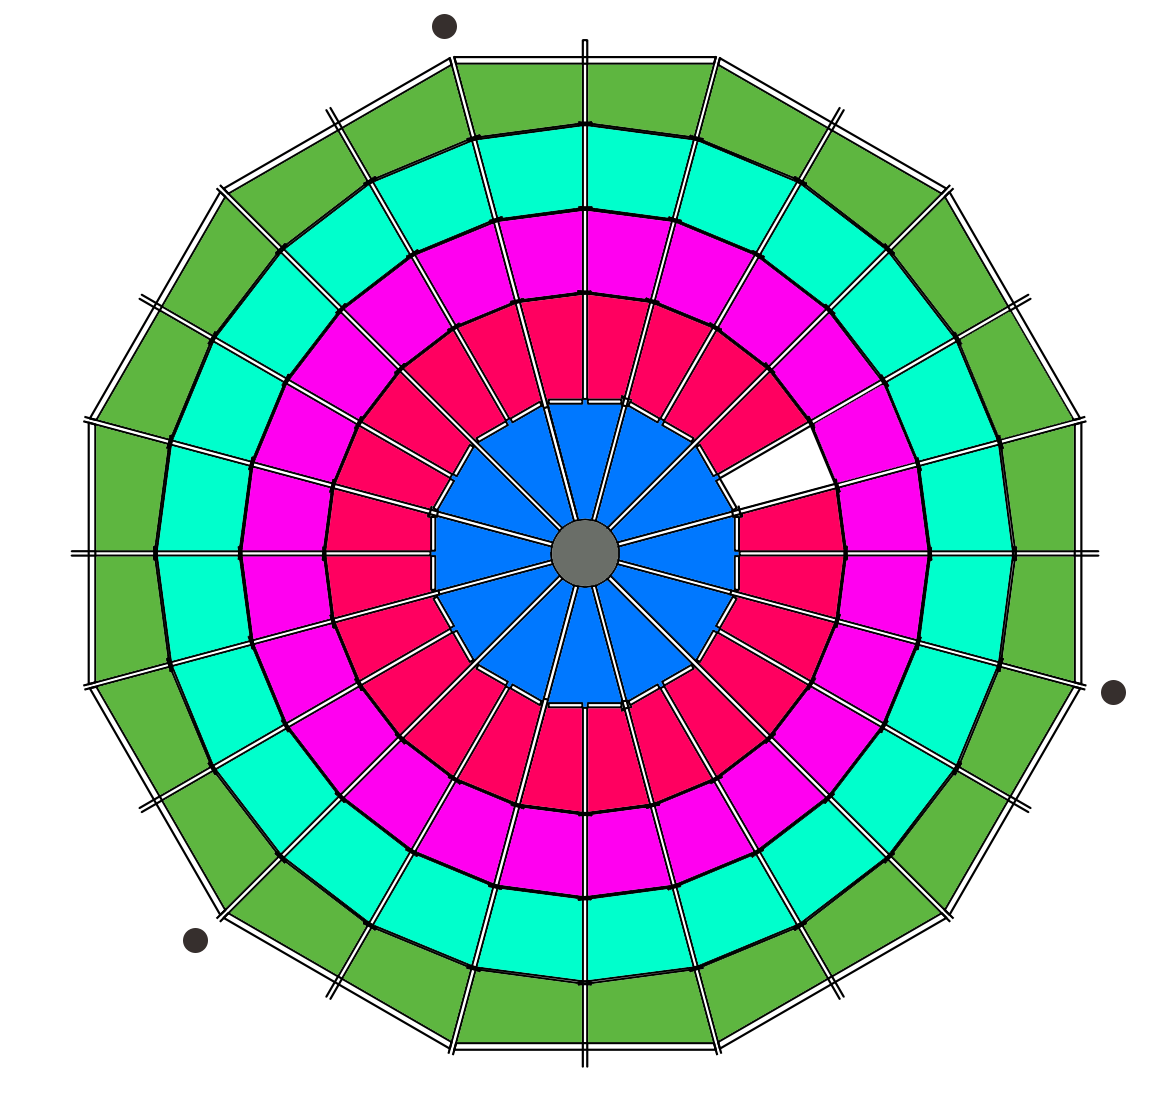
\includegraphics[width=0.5\textwidth]{antPlan.png}
\centering
\vspace{-.15in}
\caption{Panel plan.}
\label{fig:antplan}
\end{figure}

\section{Surface Spars and Bracing}
As shown in Figure \ref{fig:antplan}, the parabolic spars and associated cross bracing support the mesh.  The A-B panel overlap has a PVC cross-brace (``cross-piece''), which all holds the inner end of the intermediate support spar.  The other overlaps (B-C, C-D, D-E) have a metal strap between them. The strap is on the upper side of the PVC.  The spacing is set by the size of the mesh.

The position of the cross-piece is set by the hub and the size of panel A.  Denoting the distances as 'A' - 'E' as shown in \ref{fig:panels}, we can compute the position of the {\em far} edge of the cross-piece.  Note that the mesh follows the shape of the PVC, and the planar radial value, so it is easiest to compute the parabolic path length (denoted  by $s$, where $s=0$ at $r=0$) as opposed to the radial distance.  Radial distances may be computed numerically from the path length and vice versa.  As a shortcut here, define the mapping from radius to path-length as $f(r)$ and from path-length to radius as $f^{-1}(s)$.

Since we can mark the spar while flat on the ground as opposed to pivot along a radius, we will compute in terms of path-length $s$, but specify in terms of length along the long spars ($\sigma_L$) and the short ``intermediate'' spars ($\sigma_S$).  The offsets (shown later) are $s_{oL}$ and $s_{oS}$ respectively. That is $\sigma_{\{L,S\}}(s) = s - s_{o\{L,S\}}$. 

It is also helpful to compute the radius at which the intermediate spar starts, which is denoted $r_i$ in Fig. \ref{fig:spardims}.

\subsection{Cross-Brace Spar}
The cross-brace spar is located by where panel A would end, taking the overlap in consideration.  The PVC pipe intersects the long spars on either side at an angle of 15$^o$.  The reference point on the spar is taken to be where the long side of the cross piece intersects the long spar.
\begin{figure}[H]
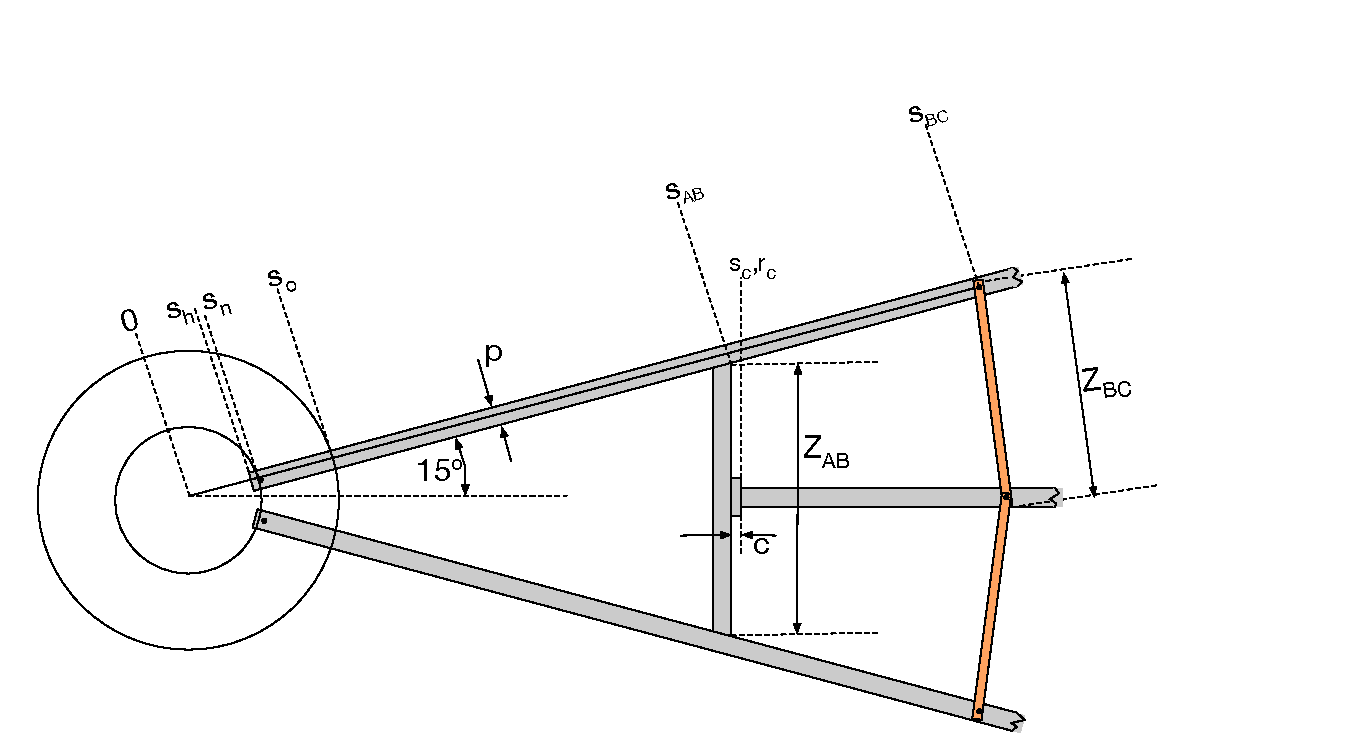
\includegraphics[width=1.0\textwidth]{spardims.pdf}
\centering
\vspace{-.15in}
\caption{Spar dimensions.}
\label{fig:spardims}
\end{figure}
\begin{equation}
\sigma_{A,L} = s_{AB} - s_h = \frac{A - \rho_o/2 + p/2}{\cos(15^o)} - \frac{p*\tan(15^o)}{2} - s_h
\end{equation}

The width of the cross-brace spar is
\begin{equation}
Z_{AB} = 2f^{-1}(s_{AB})\sin(15^o) - p/\cos(15^o)
\end{equation}

\subsection{Metal Strips}
The metal strips go between the long and short spars.  We've seen that the offset for the long is
\begin{equation}
s_{oL} = s_h
\end{equation}
and now we find
\begin{equation}
s_{oS} = s_{AB}*\cos(15^o) + c
\end{equation}
We find that the location of the metal strips are at
\begin{eqnarray}
s_{BC} & = & s_{AB} + (B - \rho_o)/\cos(7.5^o) \\
s_{CD} & = & s_{BC} + (C - \rho_o)/\cos(7.5^o) \\
s_{DE} & = & s_{CD} + (D - \rho_o)/\cos(7.5^o) \\
\end{eqnarray}
The spar markings can be found by subtracting $s_{oL}$ or $s_{oS}$ as appropriate.

The length of the metal strips
\begin{equation}
Z_{x} = 2f^{-1}(s_{x})\sin(7.5^o) + p/\cos(7.5^o)
\end{equation}
where $x = [BC,CD,DE]$

\newpage
\section{Central Feed Line Ropes}
The feed is tethered to the hub via four ropes:  3 are identical loops that loop on the feed, then the fourth gathers them below the feed and attaches to the hub.  
The feed loops between eyelets on the supporting feed triangle.  The rope lengths are chosen such that all four lengths are the same.  Figure \ref{fig:feedlinelen} sketches the overall dimensions.

\begin{figure}[H]
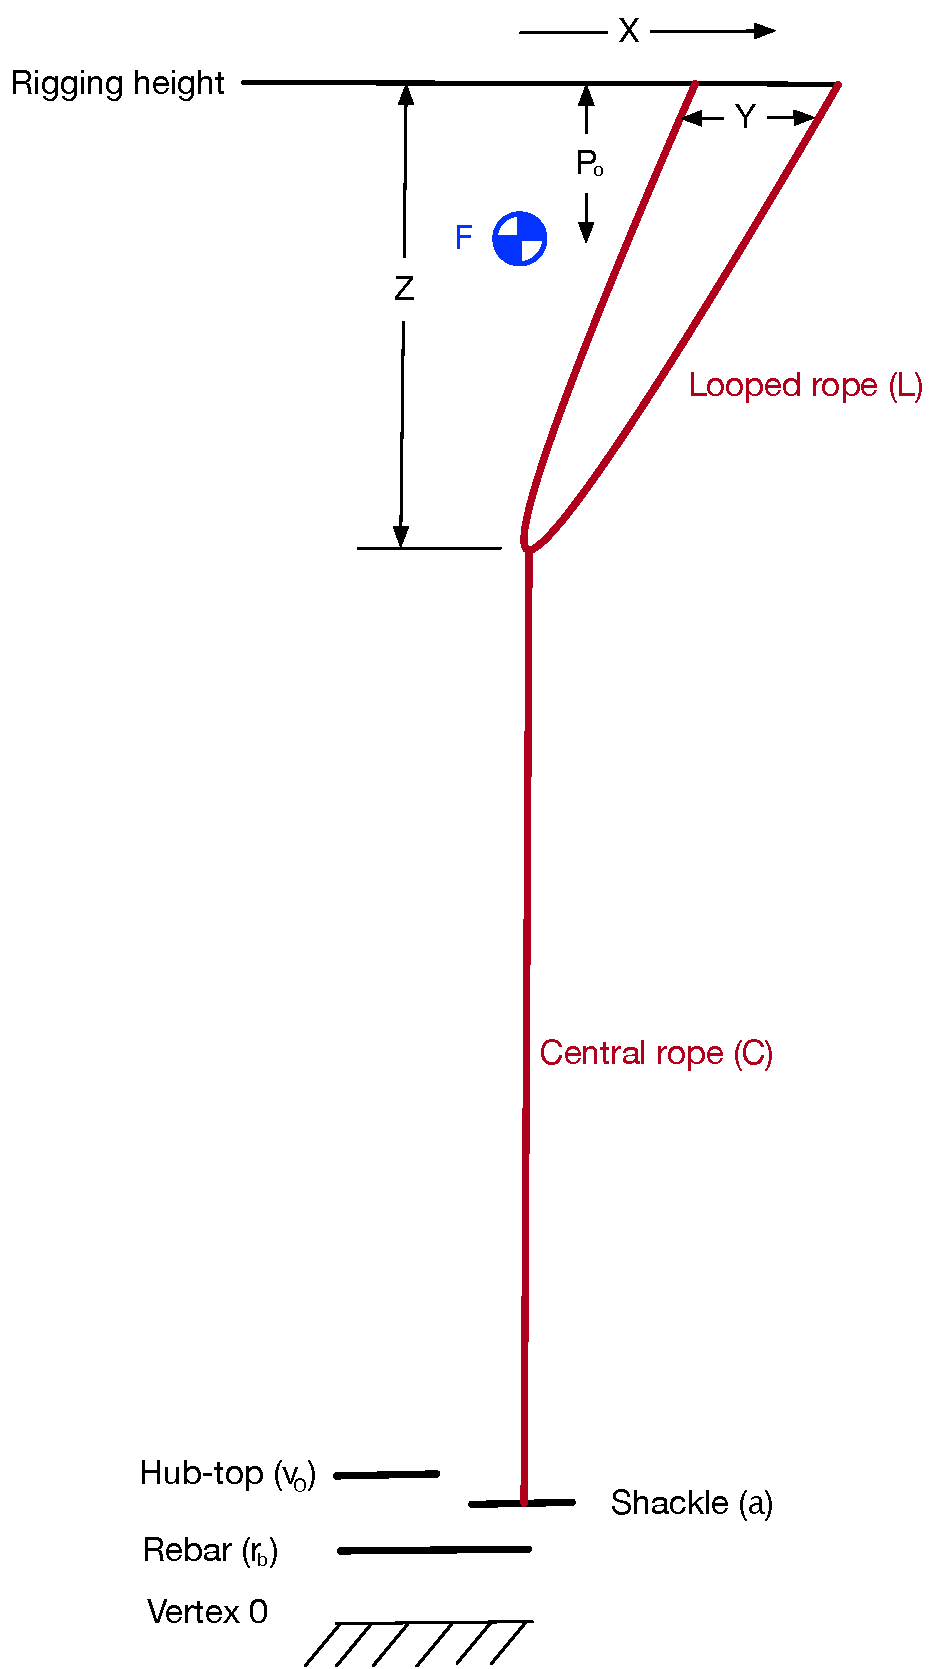
\includegraphics[width=0.3\textwidth]{feed_dims.pdf}
\centering
\vspace{-.15in}
\caption{Subset of feed locations.  In this sketch, $X$ is the projected attachment distance from the center (630 mm), $Y$ is the separation of the eye-bolts (320 mm) and $Z$ is the location where the ropes are joined.  The bottom rope attaches to the rebar with a shackle.}
\label{fig:feedlinelen}
\end{figure}

\vspace{-0.1in}
\noindent
A number of locations are defined:
\vspace{0.1in}

\begin{tabular}{l l l}
\bf{Name} & \bf{Description} & \bf{Height above vertex [mm]} \\
Vertex & Vertex of the parent parabolas & - \\
Rebar ($r_b$)  & Rebar in center of hub & 40 \\
Hub-top & Top surface of hub donut & 79 \\
Feed reference circle & PVC reference circle on feed support & 4498\\
Feed rig point & Eyebolts where lines attach & 4947\\
Feed notch & Notch used as drawing reference point & 5000 \\
Focal point & Focal point of parent parabolas & 4500 \\
Phase center & Effective phase center of feed & 4500 \\
\end{tabular}
\vspace{.2in}

\noindent
A number of distances may be found:
\vspace{0.1in}

\begin{tabular}{l l l}
\bf{Name} & \bf{Description} & \bf{Length [mm]} \\
$X$ & Projected eyebold distance from center & 630 \\
$Y$ & Eyebolt separation & 320 \\
Focal length ($F$) & Distance between vertex and focal point & 4500 \\
Rigging height & Distance between hub-top and rigging point & 4868\\
Reference height & Distance between hub-top and feed reference circle & 4419 \\
Phase center offset ($P_o$) & Distance between phase center and feed rigging point & 447 \\
Shackle offset (a) & Distance offset from shackle & 20\\
\end{tabular}
\vspace{0.1in}

And finally the rope lengths may be calculated.  Note that for convenience, it is useful to have all rope lengths be the same (and fortunately that works out to a convenient length).  For the ropes there are two lengths of interest.  First is the loop-to-loop length (the relevant length in the calculations).  Secondly is to add on the appropriate extra length needed to make the loops (taken to be 2 $\times$ 250 mm).  The total rope length is the sum.  For the bottom central rope, note that
\begin{equation}
F = r_b + a + C + Z - P_{o}
\end{equation}
so the loop-to-loop length ($C$) is
\begin{equation}
C = (F - r_b - a + P_o) - Z
\end{equation}
The loop-to-loop length for the other rope is:
\begin{equation}
L = 2\sqrt{X^2 + Y^2 + Z^2}
\end{equation}

These may be equated to yield the value for the loop-to-loop rope length:
\begin{equation}
 C = L = \frac{4K - 2\sqrt{K^2 - 3(X^2 + Y^2)}}{3}
\end{equation}
where $K = F - r_b - a +P_o$.  This yields
\vspace{.1in}

\begin{tabular}{l l}
loop-to-loop length & 3362 mm\\
total tail length & 500 mm \\
{\bf total rope length} & {\bf 3862 mm} \\
\end{tabular}

\end{document}
